Though testing for different variables, certain charactersistics were common to both cs3 {\&} cs4.
A brief list of these common variables is described in the following section.

\subsubsection{Wind Turbine Specifications} \label{sec:turb}
	We used the IEA 10 MW offshore reference turbine\cite{NREL335MW} in cs3 \& cs4, since the wind farm scenarios are modelled after an offshore location.
	This turbine's attributes are open source, and the turbine is designed as baseline for offshore wind turbine specifications.
	The power curve for the IEA 10 MW turbine is defined as shown in \cref{eq:power,fig:10MW}.
	The turbine specifications necessary for our simplified version of Bastankhah's Gaussian wake model used in cs3 are shown in \cref{tab:turb-att}.
	\begin{equation}\label{eq:power}
		P(V) = 
		\begin{cases} 
			0 & V < V_{\textit{cut-in}} \\
			P_{\textit{rated}}\bigg(\frac{V-V_{\textit{cut-in}}}{V_{\textit{rated}}-V_{\textit{cut-in}}}\bigg)^3 & V_{\textit{cut-in}}\leq V < V_{\textit{rated}} \\
			P_{\textit{rated}} & V_{\textit{rated}} \leq V < V_{\textit{cut-out}} \\
			0 & V \geq V_{\textit{cut-out}}
		\end{cases}
	\end{equation}
	%
	\begin{figure}[H]
	    \centering
	    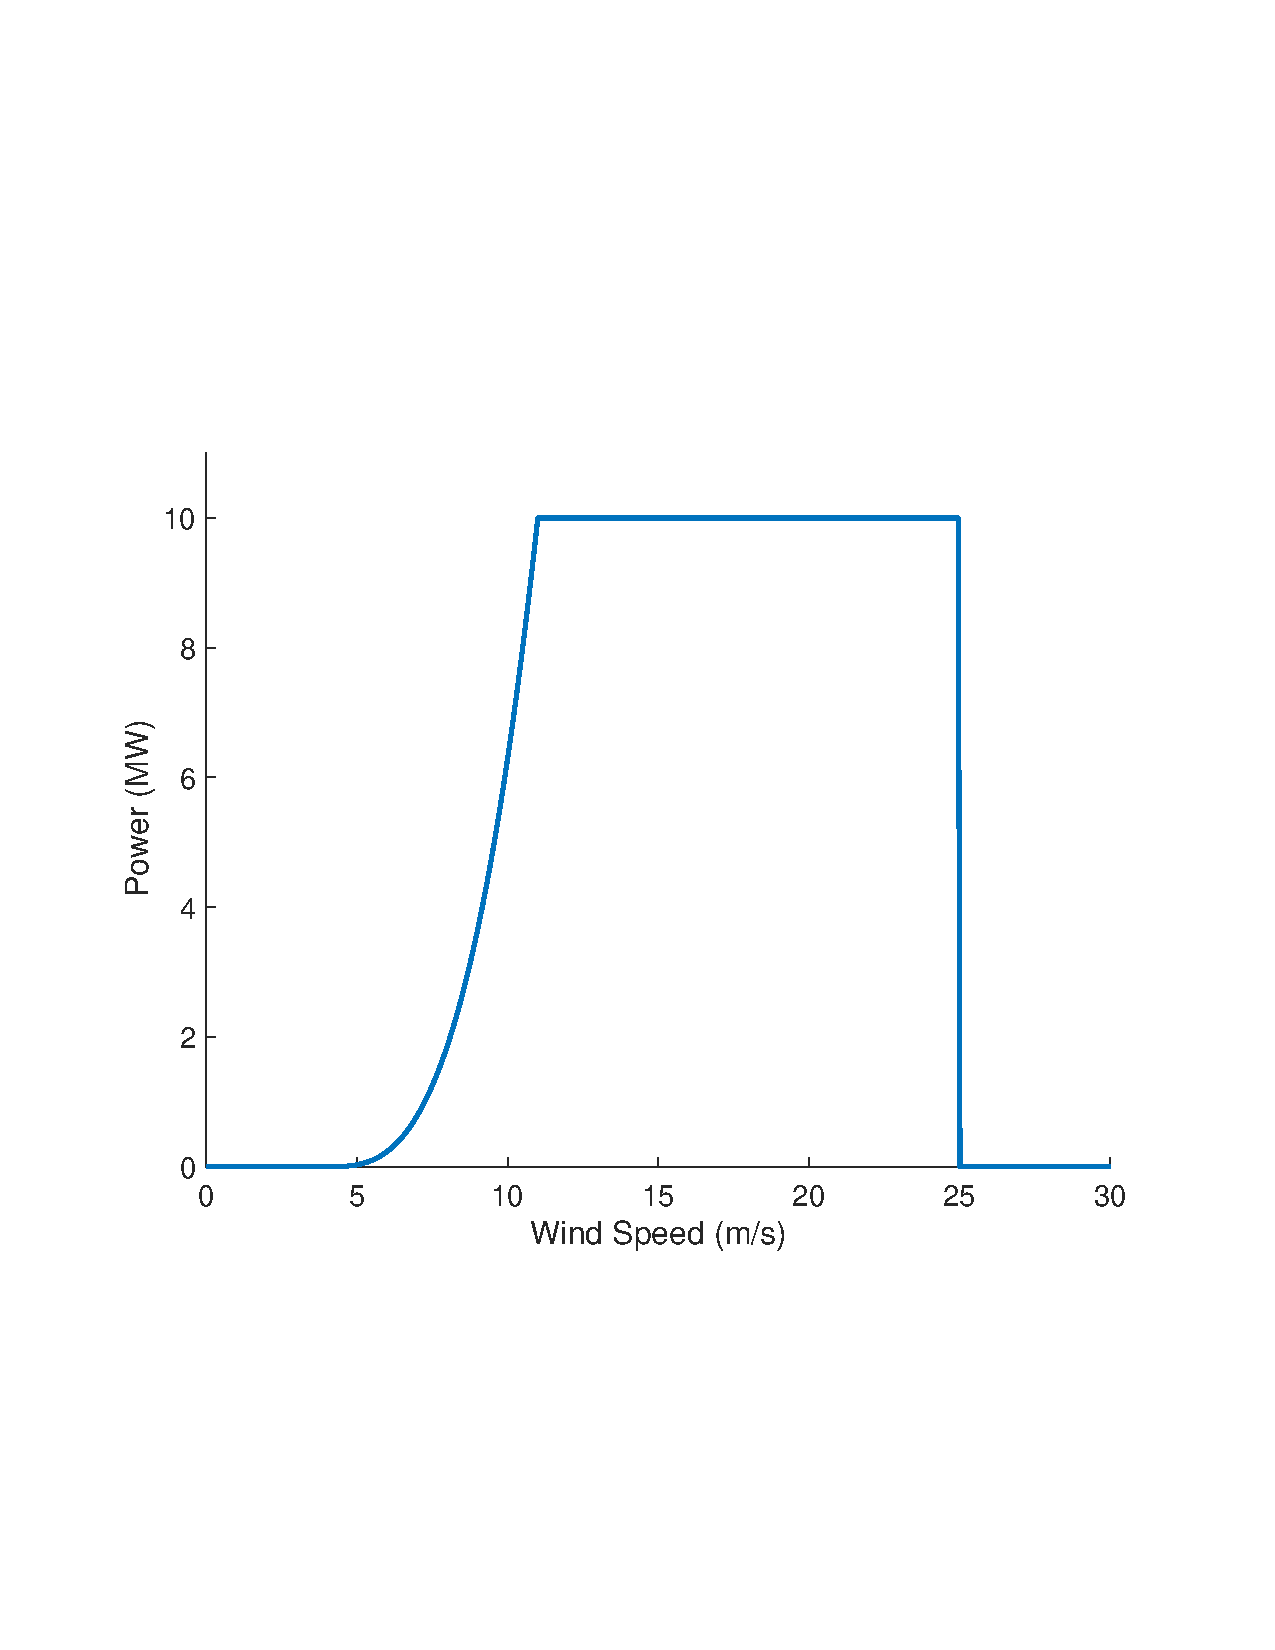
\includegraphics[width=4.0in, trim=0.8in 2.5in 1.0in 2.9in, clip]{./figures/iea37-10mw-pcurve.pdf}
	    \caption{Graphical depiction of IEA's 10-MW onshore reference turbine's power curve.}
	    \label{fig:10MW}
	\end{figure}
	%
	\begin{table}[H]
		\begin{center}
			\caption{Attributes for IEA's 10-MW onshore reference turbine}
			\label{tab:turb-att}
			\begin{tabular}{@{}lrl@{}}
			\toprule
				Rotor Diameter & 198 & m \\ 
				Turbine Rating & 10 & MW \\ 
				Cut-In Wind Speed & 4 & m/s \\ 
				Rated Wind Speed & 11 & m/s \\ 
				Cut-Out Wind Speed & 25 & m/s \\
			\bottomrule
			\end{tabular}
		\end{center}
	\end{table}
	
\subsubsection{Farm Geography}\label{sec:farmgeog}

	To focus on optimization method and EWM variability, as well as to avoid introducing too many unnecessary variables, the wind farms for all scenarios were on flat and calm seas.
%\subsubsubsection{Boundary Shape}
	Our version of the Borssele farm geography was adapted from coordinates supplied by an open solicitation for bids announced in August of 2016 by the Netherlands Enterprise Agency (NEA)\cite{BorsseleAnnouncement}.
	%The announcement document  supplied coordinates for the regions open for project design bids.
	There are neighboring farm sections already built (in the grayed out area in figure Fig.~\ref{fig:farmoutline}), but for our purposes we only utilize portions III and IV, disregarding neighboring allottments to reduce complexity.

	Top performers from cs1 \& cs2 used gradient based optimization methods, and in hindsight the simplicity of farm geography in those case studies may have favored such methods.
	The selection of the Borssele geography was in part to give difficulty to the successful methods from cs1 \& cs2, through both concavities and non-contigous regions.

	For cs1 \& cs2, the number of turbines for each increasing farm diameter were all prime numbers.
	Sticking with this theme, in cs3 \& cs4 we again chose a prime number of turbines.
	However initial tests demonstrated that, with the 10MW turbine, eighty-one (81) turbines would be too sparse a farm for interesting wake effects.
	Instead of increasing the number of turbines beyond this (which may have prohibitively increased the computational requirements for some participants), we scaled down the boundary proportions by about half, which gave us a density we felt would deliver interesting optimization results.

	As a further alteration, the original Borssele announcement required that turbine radii be contained entirely within the boundary.
	To accommodate this requirement, yet also give our participant optimizers less math to compute, boundaries were again altered inwardly by the 10MW turbine's radius, meaning that now turbine $(x, y)$ hub locations could be anywhere on or whithin the supplied boundary limits.
	As a final turbine constraint, we further mandated that turbines must be placed no less than two rotor diameters apart from any other turbine.

%%textbf{Example Layouts}
	A single example layout for each case study was supplied (displayed in Fig.~\ref{fig:ex4}), meant to give a baseline AEP output for which all participants could optimize beyond.
	The placement was largely automated to be an evenly spaced grid contoured to the boundaries, but for certain spots giving difficulty (like outcroppings), turbines were placed by hand by the author.
	This layout only serves as an AEP measure by which participant submissions can be judged so as to determine relative target function improvement.
	Participants are not required to use these layouts as starting points for their optimizations, though they have the option to do so.

\subsubsection{Wind Attributes}
	%
	\begin{figure}[]
		\begin{center}
		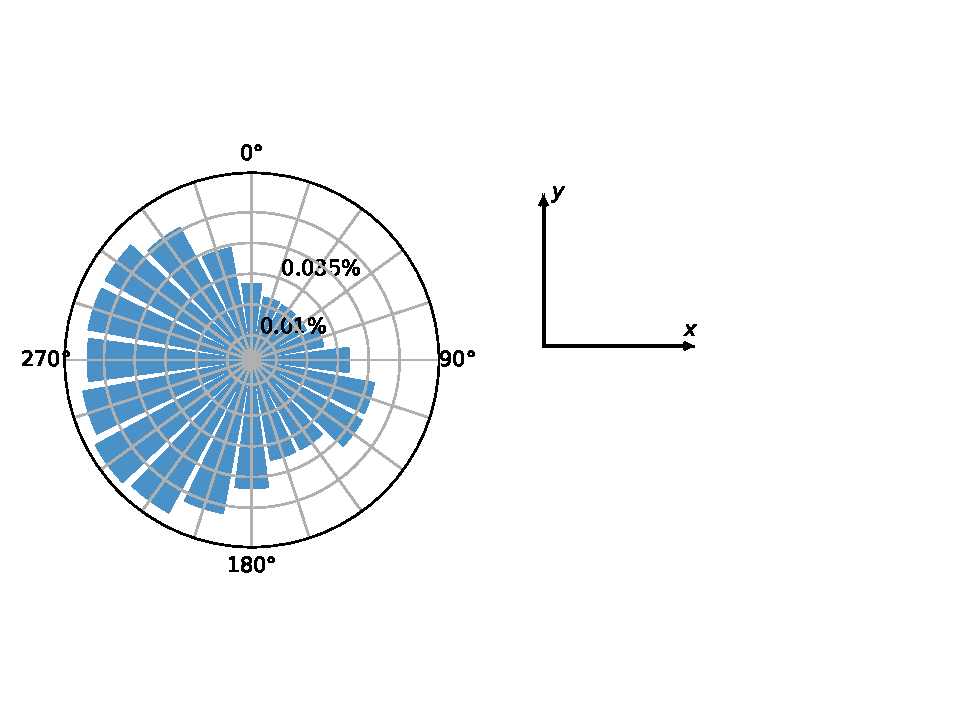
\includegraphics[width=3.25in, trim={.1in .8in 0.8in .8in},clip]{./figures/iea37-windrose.pdf}
		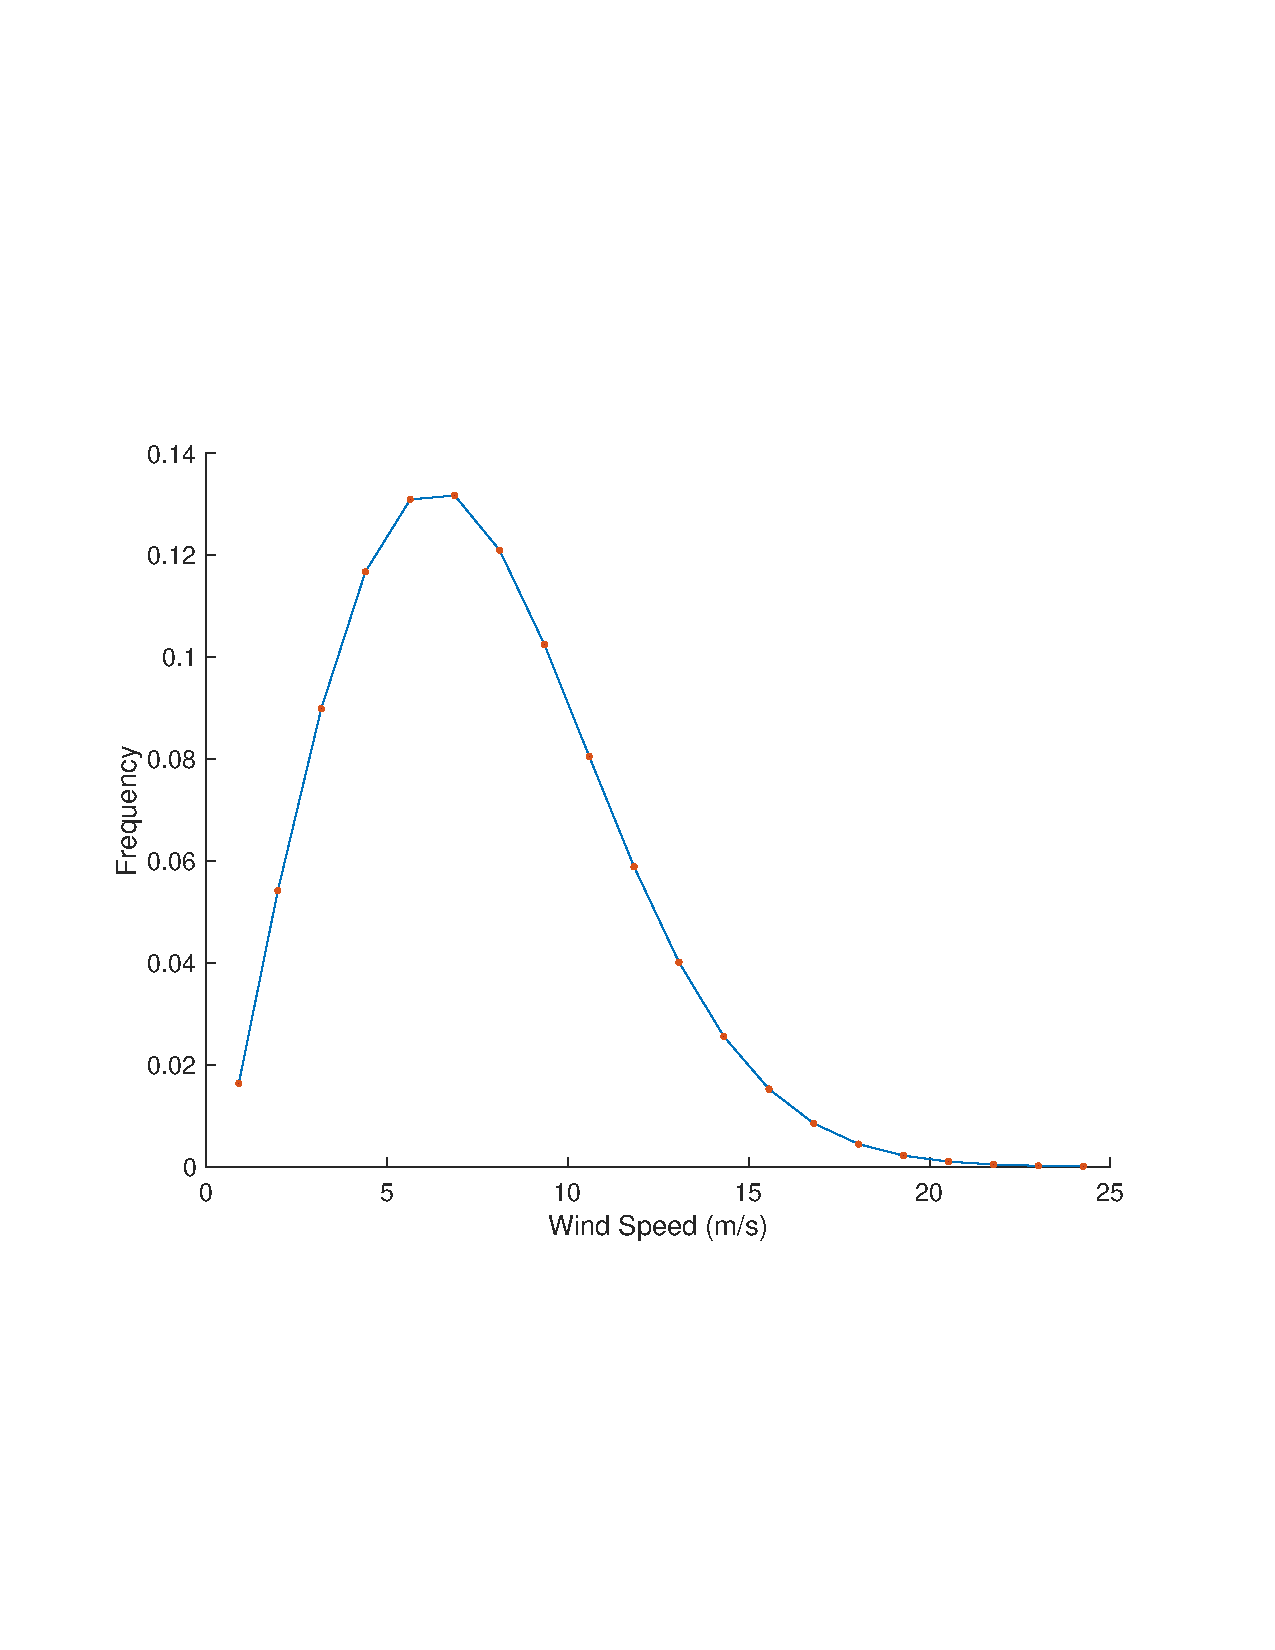
\includegraphics[width=3in, trim={.6in 2.72in 1in 2.4in},clip]{./figures/windspeed-freq.pdf}
		\captionof{figure}{(left) Wind frequency distribution over the 20 bins for the windrose used in cs3 and cs4. (right) Wind speed frequency distribution at one of the wind directions (30$^\circ$).}
		\label{fig:windrose}
		\end{center}
	\end{figure}
	%
	After completing a convergence study, we found resonable convergence in AEP calculation occured using no more than 20 wind directional bins.
	This study did not run optimizations from these differing number of bins, it simply analyzed single target function calculations.
	Had we run optimizations with varying bin numbers, we may have found more bins to have be necessary, but that can be explored in future work.
	
	The frequency distribution for each of our 20 bins is depicted graphically in polar coordinates on the left side of Fig.~\ref{fig:windrose}. 
	In this figure, a greater magnitude in the radial direction from the origin indicates a higher wind frequency from that specific direction.
	Each of the 20 binned directions have a unique frequency distribution that follows a Weibull curve, discretized for 20 values.
	An example frequency distribution for the direction of 30$^{\circ}$ is depicted on the right side of Fig.~\ref{fig:windrose}.